\documentclass{article}
\pagenumbering{arabic}
\usepackage{graphicx,amsmath,amssymb,bm,tikz}
\usetikzlibrary{calc,patterns,decorations.pathmorphing,decorations.markings}
\usepackage{xfrac}
\usepackage[utf8]{inputenc}
\usepackage{hyperref}
% Format fref 
\usepackage[plain,english]{fancyref}
\usepackage[margin=1in]{geometry} 
\fancyrefaddcaptions{english}{\renewcommand*{\frefeqname}{Eq.}}
% Figure Packages
\usepackage[outercaption]{sidecap}
\usepackage[export]{adjustbox}
\usepackage{graphicx}
\usepackage{caption}
\usepackage{wrapfig}
\usepackage{booktabs}
\newcommand{\ra}[1]{\renewcommand{\arraystretch}{#1}}
\usepackage{float}
\usepackage{algorithm, algorithmic, amsfonts,amsmath,amssymb,amsthm, color,comment,enumitem, environ, fancyhdr,   graphicx, mathtools, wasysym}
\pagestyle{fancy}
\setlength{\headheight}{22.5pt}
\newenvironment{problem}[2][Problem]{\begin{trivlist}
\item[\hskip \labelsep {\bfseries #1}\hskip \labelsep {\bfseries #2.}]}{\end{trivlist}}
\newenvironment{sol}
    {\emph{Solution:}
    }
    {
    \qed
    }
\specialcomment{com}{ \color{blue} \textbf{Comment:} }{\color{black}} %for instructor comments while grading
\NewEnviron{probscore}{\marginpar{ \color{blue} \tiny Problem Score: \BODY \color{black} }}
\usepackage{etoolbox}
% Page rotation
\makeatletter
\def\ifGm@preamble#1{\@firstofone}
\appto\restoregeometry{%
  \pdfpagewidth=\paperwidth
  \pdfpageheight=\paperheight}
\apptocmd\newgeometry{%
  \pdfpagewidth=\paperwidth
  \pdfpageheight=\paperheight}{}{}
\makeatother
%%%%%%%%%%%%%%%%%%%%%%%%%%%%%%%%%%%%%%%%%%%%%%%%%%%%%%%%%%%%%%%%%%%%%%%%%%%%%%%%%





%%%%%%%%%%%%%%%%%%%%%%%%%%%%%%%%%%%%%%%%%%%%%
%Fill in the appropriate information below
\lhead{Agramonte, Heydari}  %replace with your name
\rhead{ENGR 8990 \\ Project 1 - Lesson 1} %replace XYZ with the homework course number, semester (e.g. ``Spring 2019"), and assignment number.
%%%%%%%%%%%%%%%%%%%%%%%%%%%%%%%%%%%%%%%%%%%%%



% Table stuff
\usepackage{multirow}
%\usepackage{floatrow}
%	\floatsetup[table]{capposition=top}%puts table caption above
% Change \subsection title characteristics
    \usepackage[parfill]{parskip}   % forces parskip to not affect headings
    \usepackage{enumitem}           % used for editing itemize environment
    \usepackage{titlesec}
        \titleformat*{\section}{\Large\bfseries\titlerule\vspace{0.5em}}
% Quote blocks
    \usepackage{csquotes} % use environment 'displayquote'
% Misc document settings
    \title{\Huge ENGR 8990 Project 1 - Lesson 1} \author{Daniel Agramonte, Mahtab Heydari} \date{12.05.20}
    \setlength{\parindent}{0pt}
    \setlength{\parskip}{1em}
    \setlist{nosep, itemsep=0pt, parsep=0pt}
% Misc vocab commands
    \newcommand{\msalg}{{\fontfamily{cmtt}\selectfont ms83}}
    \newcommand{\lsq}{\emph{lsqnonlin}}
    \newcommand{\msalge}{{\fontfamily{cmtt}\selectfont MCHE\_6500\_NIST\_POLY}}
%
% MATLAB packages
%
\usepackage[framed,numbered]{matlab-prettifier}
\usepackage{textcomp}
\usepackage{listings}
%
% Matrix Spacing
%
\makeatletter
\renewcommand*\env@matrix[1][\arraystretch]{%
  \edef\arraystretch{#1}%
  \hskip -\arraycolsep
  \let\@ifnextchar\new@ifnextchar
  \array{*\c@MaxMatrixCols c}}
\makeatother
%
\begin{document}
\maketitle

Product: Electronic keyboard for recreational, educational, and professional use 
\begin{table}[H]
    \centering
    \begin{tabular}{|p{2cm}||p{2cm}|p{2cm}|p{1.5cm}|p{2cm}|p{2cm}|}
        \hline
        & Customers & Educators & Artists & Recording Studio & Warranty Services\\
        \hline
        \hline
        Amateur & 5 & 2 & 1 & - & 2 \\
        \hline
        Professional & 5 & - & 3 & 3 & 2 \\
        \hline
        Institution & 2 & 5 & 3 & 4 & 2 \\
        \hline
    \end{tabular}
    \caption{Stakeholder Selection Matrix}
    \label{tab:Stakeholder_Selection_Matrix}
\end{table}

Customers: users/buyers of the electronic keyboard instrument
\newline
Educators: private music teachers, K-12 music educators, university instructors
\newline 
Artists: composers, songwriters, MIDI software users
\newline 
Recording Studio: sound engineers, mixers
\newline
Warranty Services: i.e. Yamaha servicer

Primary Markets: Novice Players (Amateur and Institution) \newline 
Secondary Market: Professional

\newpage
\thispagestyle{plain}
\newgeometry{,hmargin=1in,vmargin=1in,landscape}
\begin{figure}
    \vspace{-10pt}
    \centering
    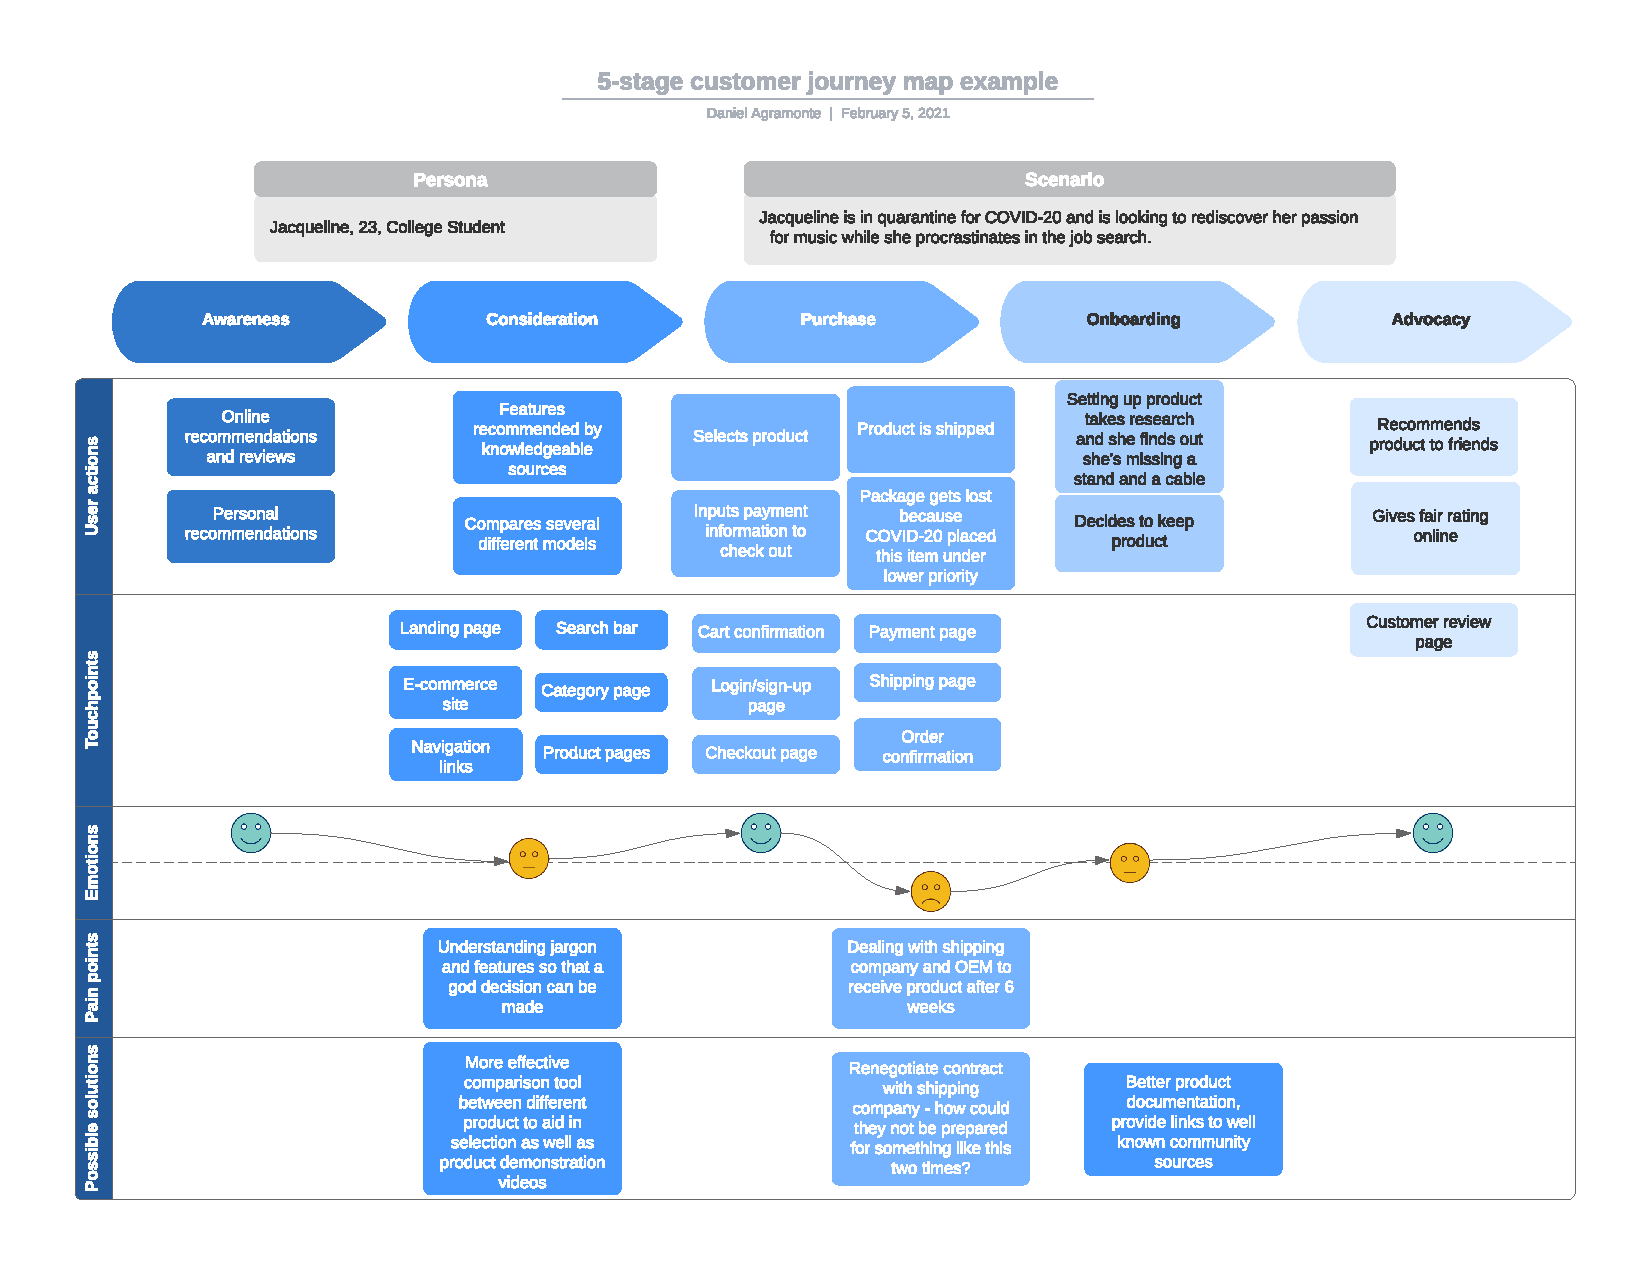
\includegraphics[trim=0 0 0 100,clip,width=\textwidth]{ENGR 8990/Projects/Project 1/Figures/5-stage customer journey map.pdf}
    \captionsetup{justification=raggedright,singlelinecheck=false}
    \caption{Customer Journey Map}
    \label{fig:CJM}
\end{figure}
\restoregeometry

\end{document}